\section{Application of Independent Component Analysis on Acoustic Signals via R}   


With the preprocessed data, we can proceed with the application of ICA. Note that among various algorithms for ICA, in this dissertation we focus on using the \emph{fastICA}. In R language we would use the function \emph{fastICA()} from the package \emph{fastICA}.

The code for processing ICA is much simpler than PCA; we consider the two main variables \emph{x} and \emph{n.comp} in the function \emph{fastICA}(). The variable \emph{x} holds multidimensional signal matrix (or dataframe), where each row represents observations (the signal data) and each column represents variables (sampling points). The variable \emph{n.comp} holds a numeric value, which is the number of components to be extracted through the \emph{fastICA}() function \cite{fastICACranR}. 

We simply put variable \emph{x} as the interpolated dataframe \emph{finalDF} and adjust the variable \emph{n.comp} ranging from 1 to the number of observations (in our case 219), and observe the difference on the result.

We would compute the function \emph{fastICA}() with the variables as described above and store the computed result in object \emph{ica\textbf{n}}, where \textbf{n} would be the value of the variable \emph{n.comp}. The object \emph{ica\textbf{n}} consists of five elements \emph{X, K, W, A, S}, where each element represents the step-by-step result of the process. 

Element \emph{X} is the pre-processed data matrix of 219 rows (number of observed signals) and 5000 columns (number of sampling points). 

Element \emph{K} is the pre-whitening matrix that projects data onto the first \emph{n.comp} principal components. It consists of 5000 rows (number of sampling points) and \emph{n.comp} columns.

Element \emph{W} is the estimated un-mixing matrix of \emph{n.comp} rows and \emph{n.comp} columns.

Element \emph{A} is the estimated mixing matrix of \emph{n.comp} rows and 5000 columns (number of sampling points).

And finally, element \emph{S} is the estimated source matrix of \emph{n.comp} rows and 5000 columns (number of sampling points). The data in element \emph{S} is the information that we would want to use. 

We would first start with \emph{n.comp} value of 5 and observe the outcome. The computed value would be stored on object \emph{ica5}. The following figure shows the combinations of biplots between the five components from the five rows of element \emph{S} from \emph{ica5}. 

\begin{figure}[H]
    \centering
    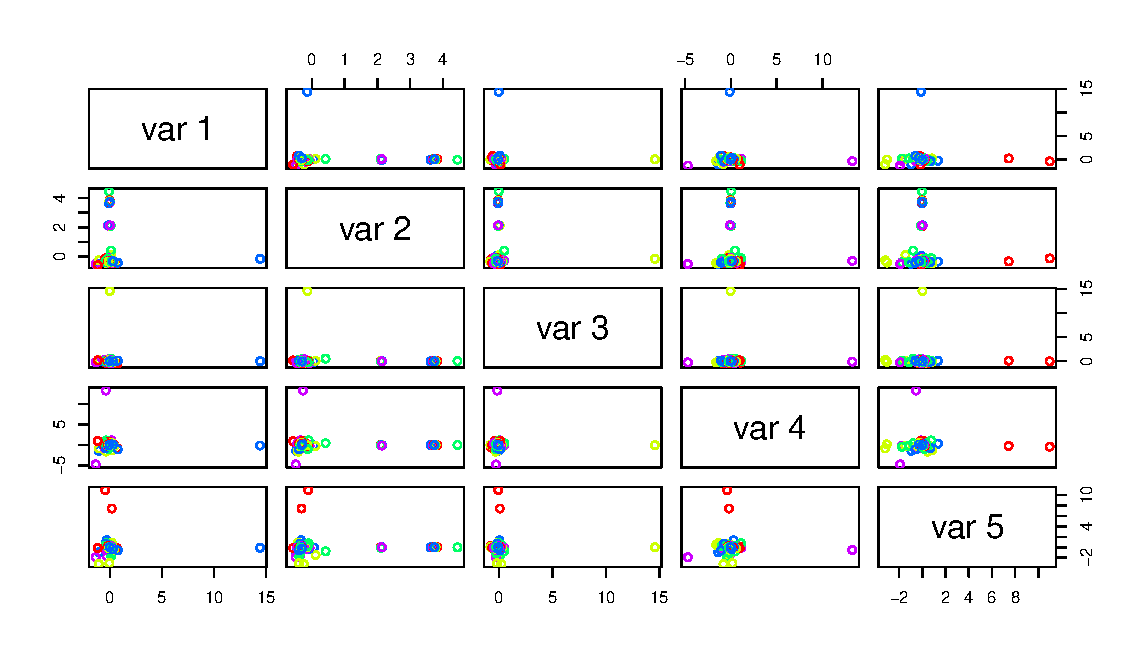
\includegraphics[width=15cm]{images/ICA/[5]/[5] 5 x 5 plot.pdf}  
    \caption{Biplots of 5 components}
    \label{fig:[5]5x5biplots]} 
\end{figure}

It is unclear to tell which component best separates the data on its own, or in other words is closest to a uniform shape, just by observing the biplots. In order to determine which component best separates the data, we can compute the difference of the 219 elements of each component to a uniform vector of same maximum and minimum value and number of points.

For each i-th component, which can be accessed as \emph{S}[,i], we calculate the sum of the absolute value of the difference between each element from a uniform matrix and the closest element from the i-th component. 

By using a \emph{for}() loop with variable \emph{j} from 1 to 219, we calculate the element of i-th component which is the closest to the j-th index element of the uniform vector. Then we calculate the absolute value of the difference of the two values. Throughout the iteration, we increment these 219 values into object \emph{uniVal}. Thus, we have the total sum of the difference \emph{uniVal} for each i-th component.

The component with the lowest \emph{uniVal} value would be the one that is the closest to a uniform distribution. Using this algorithm on data \emph{ica5}, we get a result that component 2 has the lowest \emph{uniVal} value. We can plot a representation of component 2 to observe and visually confirm the spread and variance. The following figure is a biplot with x and y axis both being component 2, \emph{S}[,2].
\begin{figure}[H]
    \centering
    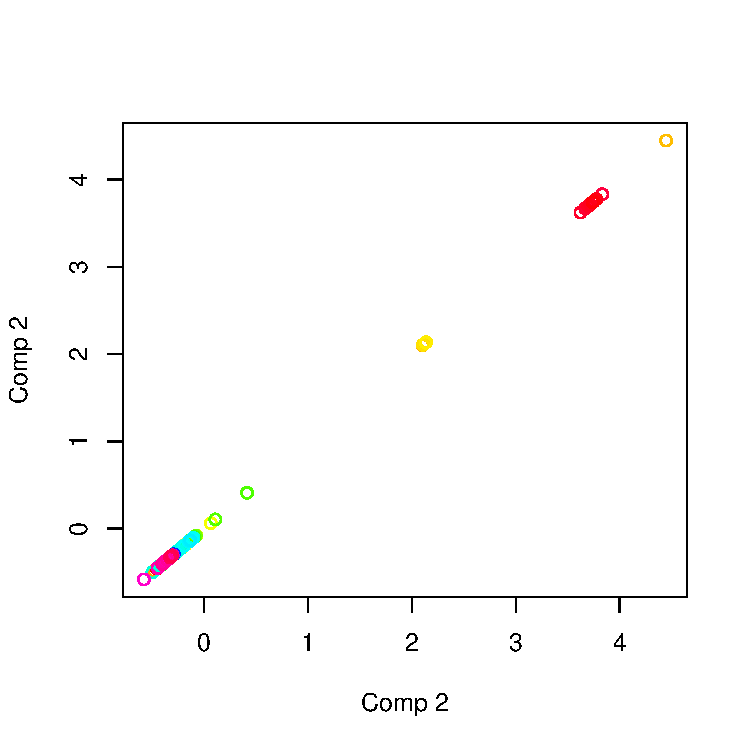
\includegraphics[width=9cm]{images/ICA/[5]/comp 2.pdf}  
    \caption{Biplot of component 2}
    \label{fig:[5]comp2} 
\end{figure}

Now we can increase the value of \emph{n.comp} and observe the difference in the result. We execute \emph{fastICA} with \emph{n.comp} set as 10 and save the computed result in object \emph{ica10}. Using the same algorithm to calculate which component best separates the data on its own, we get a result that component 19 has the lowest \emph{uniVal} value. The following figure is a biplot with x and y axis both being component 19, \emph{S}[,19].
\begin{figure}[H]
    \centering
    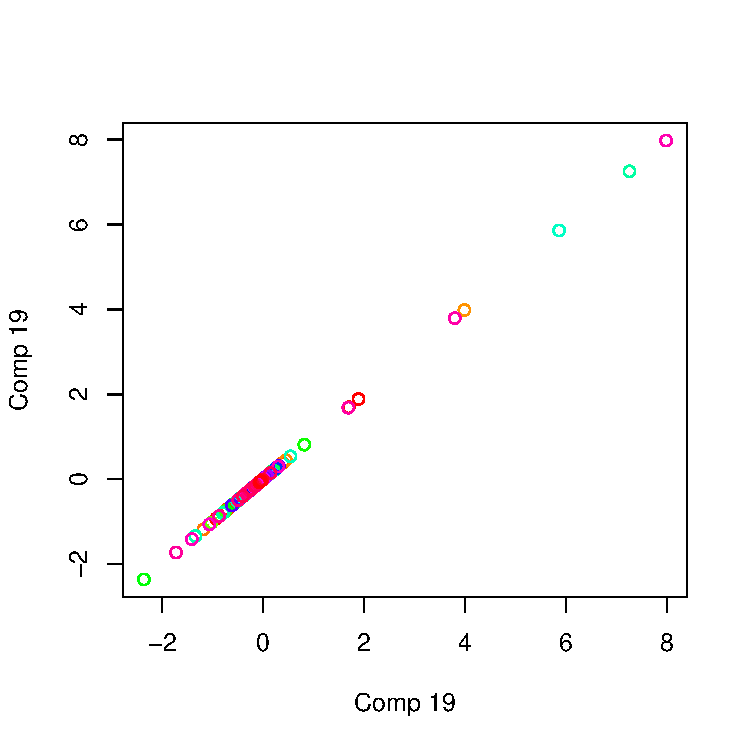
\includegraphics[width=9cm]{images/ICA/[10]/comp 19.pdf}  
    \caption{Biplot of component 19}
    \label{fig:[10]comp19} 
\end{figure}
We can notice from the figure that the plot of component 19 from \emph{ica10} is more evenly distributed and has a shape closer to a uniform vector, compared to the plot of component 2 from \emph{ica5}. From this result we can assume that increasing the value of \emph{n.comp} leads to increased number of components being produced, thus may lead to finding a better representation of component that best separates the data on its own. We would carry on with further exectuion of \emph{fastICA} with increased value of \emph{n.comp} in order to verify this assumption.

Again, we execute \emph{fastICA} with increased value of \emph{n.comp}, set to 20, and save the computed result in object \emph{ica20}. Using the same algorithm to calculate which component best separates the data on its own, we get a result that component 7 has the lowest \emph{uniVal} value. The following figure is a biplot with x and y axis both being component 7, \emph{S}[,7].
\begin{figure}[H]
    \centering
    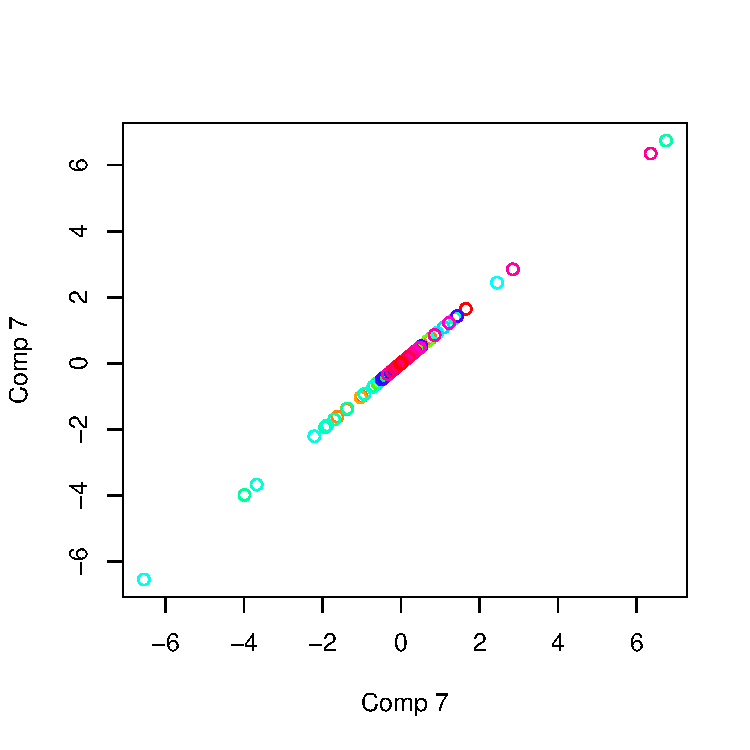
\includegraphics[width=9cm]{images/ICA/[20]/comp 7.pdf}  
    \caption{Biplot of component 7}
    \label{fig:[20]comp7} 
\end{figure}

Again, we execute \emph{fastICA} with increased value of \emph{n.comp}, set to 40, and save the computed result in object \emph{ica40}. Using the same algorithm to calculate which component best separates the data on its own, we get a result that component 13 has the lowest \emph{uniVal} value. The following figure is a biplot with x and y axis both being component 13, \emph{S}[,13].
\begin{figure}[H]
    \centering
    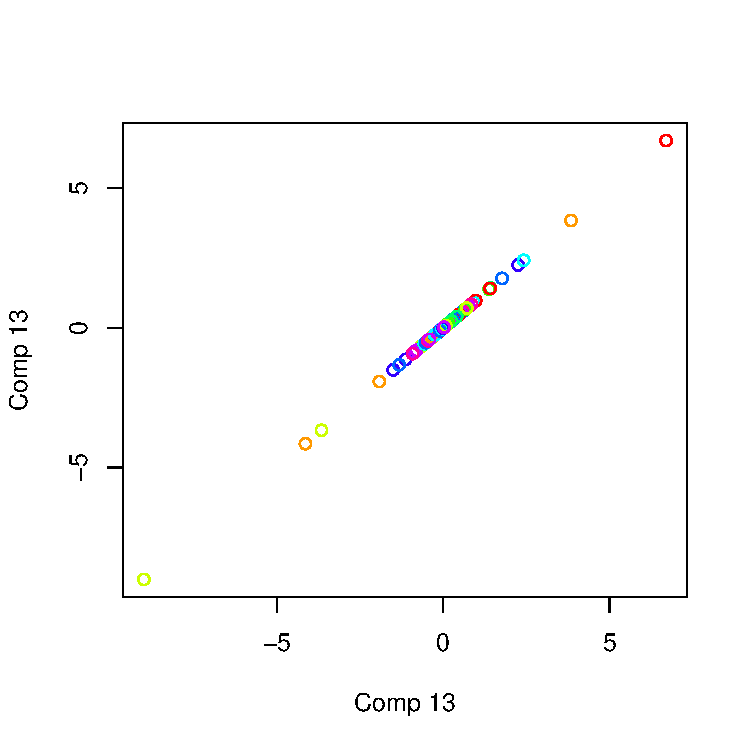
\includegraphics[width=9cm]{images/ICA/[40]/comp 13.pdf}  
    \caption{Biplot of component 13}
    \label{fig:[40]comp13} 
\end{figure}

We execute our last process of \emph{fastICA} with increased value of \emph{n.comp}, set to 80, and save the computed result in object \emph{ica80}. Using the same algorithm to calculate which component best separates the data on its own, we get a result that component 50 has the lowest \emph{uniVal} value. The following figure is a biplot with x and y axis both being component 50, \emph{S}[,50].
\begin{figure}[H]
    \centering
    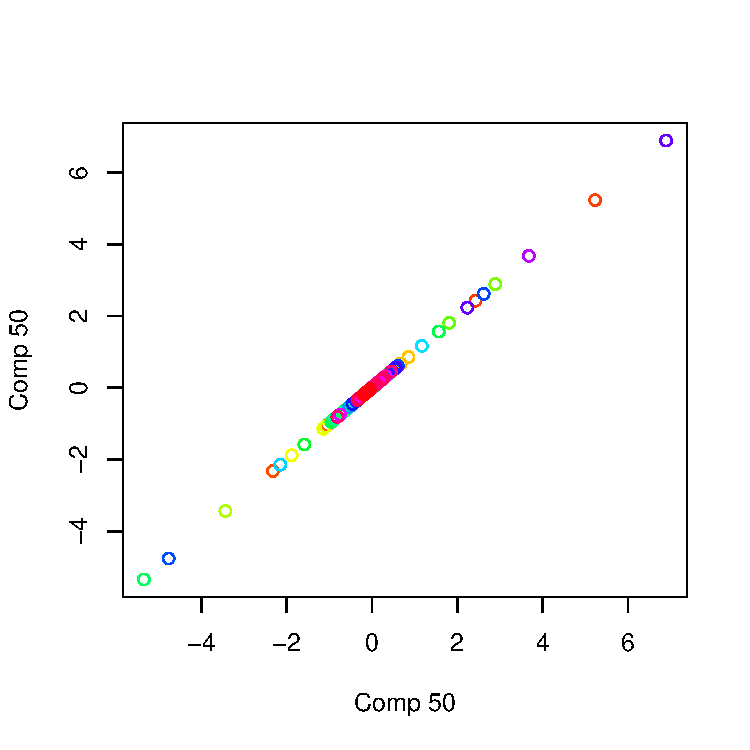
\includegraphics[width=9cm]{images/ICA/[80]/comp 50.pdf}  
    \caption{Biplot of component 50}
    \label{fig:[80]comp50} 
\end{figure}

By comparing the five biplots of the best separating components from each processed data \emph{ica5, ica10, ica20, ica40, ica80}, we can observe that throughout each iteration, as the value set for \emph{n.comp} increases, the plot forms closer to a uniform vector.

In conclusion we have applied the \emph{fastICA} algorithm on interpolated 219 acoustic signal data with five different values selected for the number of components. We have made an assumption that as the number of components calculated increases, the more likely we could find a component that well-separates the data on its own. Throughout the 5 calculations, from 5 components to 80 components, we have visually observed through the biplots of the components that our assumption holds valid.

Application of \emph{fastICA} on spectrum dataframe could not have been performed due to the exhausting time complexity of the data. This aspect also shows the inefficiency of ICA algorithms, when it is used with the goal to reduce the dimension of acoustic signal data with large number of sampling points (in other words variables), rather than to separate independent sources from a mixed signal. 